\documentclass[11pt]{article}
\usepackage[margin=1in]{geometry}
\usepackage[T1]{fontenc}
\usepackage{lmodern}
\usepackage{amsmath,amssymb}
\usepackage{booktabs}
\usepackage[numbers,sort&compress]{natbib}
\usepackage[hidelinks]{hyperref}
\usepackage{graphicx}
\usepackage[font=footnotesize,skip=3pt]{caption}
\sloppy
\setlength{\bibsep}{1.5pt}
\setlength{\textfloatsep}{10pt plus 2pt minus 2pt}
\setlength{\floatsep}{8pt plus 2pt minus 2pt}

% Every measured figure in the prose is a macro from generated/numbers.tex, which
% build_assets.py writes from docs/validation/*.json. See tests/test_paper.py.
% Generated by paper/build_assets.py from docs/validation/*.json. Do not edit.
\newcommand{\accMatChamp}{0.4338}
\newcommand{\accMatDS}{0.9487}
\newcommand{\bestPrompt}{$-$0.0701}
\newcommand{\bestPromptAbs}{0.0701}
\newcommand{\bestPromptHi}{$-$0.0481}
\newcommand{\bestPromptLo}{$-$0.0936}
\newcommand{\ciPct}{95}
\newcommand{\ckptPoolTasks}{200}
\newcommand{\ckptRho}{$-$0.608}
\newcommand{\ckptSpread}{0.259}
\newcommand{\ckptSpreadX}{8.99}
\newcommand{\combEffect}{+0.0970}
\newcommand{\combEffectHi}{+0.1250}
\newcommand{\combEffectLo}{+0.0724}
\newcommand{\costSeedLow}{0.267}
\newcommand{\costSeedMidHigh}{0.150}
\newcommand{\costSeedMidLow}{0.167}
\newcommand{\costShipped}{0.000}
\newcommand{\decodeSamples}{5}
\newcommand{\decodeTemp}{0.6}
\newcommand{\dedupShift}{0.0006}
\newcommand{\devPoolSeed}{13}
\newcommand{\devPoolSeedList}{7, 13, 42}
\newcommand{\dsRw}{0.8719}
\newcommand{\evalPoolOverMargin}{0.40}
\newcommand{\evalPoolRange}{0.0230}
\newcommand{\exactOverlap}{0}
\newcommand{\fOneChamp}{0.824}
\newcommand{\fOneDS}{0.904}
\newcommand{\fOneMatChamp}{0.6649}
\newcommand{\fOneMatDS}{0.9604}
\newcommand{\floorAcc}{0.0912}
\newcommand{\floorRw}{0.6673}
\newcommand{\fpChamp}{67}
\newcommand{\fpDS}{0}
\newcommand{\freshGapToDS}{0.0716}
\newcommand{\freshMax}{0.8353}
\newcommand{\freshSDoverMargin}{1.66}
\newcommand{\frozenSeed}{999}
\newcommand{\highRecall}{1.000}
\newcommand{\lossAfter}{0.111}
\newcommand{\lossBefore}{0.117}
\newcommand{\margin}{0.0288}
\newcommand{\marginXthree}{0.0409}
\newcommand{\matMargin}{$-$0.0288}
\newcommand{\matMarginHi}{$-$0.0160}
\newcommand{\matMarginLo}{$-$0.0432}
\newcommand{\nBench}{800}
\newcommand{\nCkpt}{14}
\newcommand{\nClean}{419}
\newcommand{\nExc}{381}
\newcommand{\nFrozen}{800}
\newcommand{\nHigh}{184}
\newcommand{\nMidBand}{771}
\newcommand{\nPoolTasks}{300}
\newcommand{\nSeedFresh}{3}
\newcommand{\nSeedRuns}{4}
\newcommand{\nTrain}{3198}
\newcommand{\nearDup}{29}
\newcommand{\nearDupPct}{3.62}
\newcommand{\nnFloor}{0.6}
\newcommand{\nnHigh}{0.8}
\newcommand{\pFresh}{0.12}
\newcommand{\partialChamp}{22}
\newcommand{\partialContrib}{0.0322}
\newcommand{\partialDS}{5}
\newcommand{\partialN}{32}
\newcommand{\partialShare}{112}
\newcommand{\partialShareXthree}{97}
\newcommand{\plateauN}{4}
\newcommand{\plateauSpread}{0.0665}
\newcommand{\plateauSpreadX}{2.31}
\newcommand{\pmPairs}{9}
\newcommand{\pmShared}{9}
\newcommand{\pmTableSize}{10}
\newcommand{\poolMeanShift}{0.0334}
\newcommand{\poolShift}{0.0444}
\newcommand{\poolShiftOverMargin}{1.54}
\newcommand{\precMatChamp}{0.5083}
\newcommand{\pubMargin}{+0.0288}
\newcommand{\pubMarginCorr}{+0.0269}
\newcommand{\pubMarginCorrHi}{+0.0493}
\newcommand{\pubMarginCorrLo}{+0.0064}
\newcommand{\pubMarginHi}{+0.0513}
\newcommand{\pubMarginLo}{+0.0074}
\newcommand{\rangeOverMargin}{6.92}
\newcommand{\resamples}{10{,}000}
\newcommand{\rescoredBase}{0.6002}
\newcommand{\rescoredChamp}{0.9007}
\newcommand{\rescoredDS}{0.8719}
\newcommand{\rescoredFP}{67}
\newcommand{\rescoredFPds}{0}
\newcommand{\rescoredMargin}{0.0288}
\newcommand{\rubricEffect}{+0.0413}
\newcommand{\rwAfter}{0.7022}
\newcommand{\rwBase}{0.6002}
\newcommand{\rwBefore}{0.8920}
\newcommand{\rwChamp}{0.9007}
\newcommand{\rwChampCorr}{0.8988}
\newcommand{\rwChampHi}{0.924}
\newcommand{\rwChampLo}{0.876}
\newcommand{\rwChampPoolBench}{0.9007}
\newcommand{\rwChampXthree}{0.9128}
\newcommand{\rwDS}{0.8719}
\newcommand{\rwDSHi}{0.899}
\newcommand{\rwDSLo}{0.843}
\newcommand{\rwEvalPoolHigh}{0.9451}
\newcommand{\rwEvalPoolLow}{0.9221}
\newcommand{\rwEvalPoolSD}{0.0115}
\newcommand{\rwFreshMean}{0.8003}
\newcommand{\rwFreshSD}{0.0479}
\newcommand{\rwFreshSDhi}{0.3010}
\newcommand{\rwFreshSDlo}{0.0249}
\newcommand{\rwMatChamp}{0.9401}
\newcommand{\rwMatDS}{0.9689}
\newcommand{\rwMean}{0.8365}
\newcommand{\rwMeanMinusSD}{0.7542}
\newcommand{\rwRange}{0.1994}
\newcommand{\rwSD}{0.0823}
\newcommand{\rwSDhi}{0.3068}
\newcommand{\rwSDlo}{0.0466}
\newcommand{\rwSDnoDecode}{0.0814}
\newcommand{\rwSDoneSided}{0.0510}
\newcommand{\rwSamplingMarginal}{0.0121}
\newcommand{\rwSeedLow}{0.7457}
\newcommand{\rwSeedMidHigh}{0.8353}
\newcommand{\rwSeedMidLow}{0.8198}
\newcommand{\rwShipped}{0.9451}
\newcommand{\rwShippedCkpt}{0.9612}
\newcommand{\rwSiblingXthree}{0.7291}
\newcommand{\rwTrainSeedGapOld}{0.1837}
\newcommand{\samplesChamp}{5}
\newcommand{\samplingOverMargin}{0.42}
\newcommand{\sdOverCorrMargin}{3.06}
\newcommand{\sdOverMargin}{2.86}
\newcommand{\seedsNeeded}{65}
\newcommand{\seedsNeededFresh}{22}
\newcommand{\shipGapFresh}{0.1448}
\newcommand{\shipGapOverMargin}{5.03}
\newcommand{\skillAccChamp}{0.5905}
\newcommand{\skillAccDS}{0.7400}
\newcommand{\skillBase}{$-$0.2017}
\newcommand{\skillChamp}{0.7015}
\newcommand{\skillDS}{0.6150}
\newcommand{\skillFOneChamp}{0.5042}
\newcommand{\skillFOneDS}{0.7283}
\newcommand{\tFresh}{$-$2.59}
\newcommand{\tempChamp}{0.6}
\newcommand{\tempDS}{0.0}
\newcommand{\voteChanges}{8}


\title{When a Small Fine-Tune's Margin Sits Inside Its Training-Seed Spread:\\
Variance Decomposition, Class Memorization, and Prompt Confounds in Financial Reconciliation}
\author{Caio Theodoro\\ \small Avenza Labs (\texttt{avenza.cloud}) \and Jo\~{a}o Vitor Basso Sberse\\ \small Avenza Labs (\texttt{avenza.cloud})}
\date{Work begun 7 August 2026; this version 23 November 2026}

\begin{document}
\maketitle

\begin{abstract}
Small fine-tuned language models are frequently reported to beat frontier models on narrow structured tasks from a single training run and a task-resampling confidence interval. We audit one such previously published claim---a 1.7B-parameter LoRA fine-tune outperforming DeepSeek v4-flash on severity-weighted recall ($R_w$) across \nBench{} synthetic financial reconciliation tasks (\rwChamp{} against \rwDS{}, margin \margin{})---against a pre-registered seed-spread rule and five independent diagnostics. First, across four runs of one recipe on a \nPoolTasks{}-task development pool, $R_w$ spans \rwSeedLow{} to \rwShipped{} (SD \rwSD{}, \sdOverMargin{} times the margin), with the shipped run at the top; across the three unselected runs trained afterwards, SD is \rwFreshSD{} (\freshSDoverMargin{} times the margin, whose \ciPct{}\% chi-square interval includes the margin) and the shipped run sits \shipGapFresh{} above their mean. Accordingly, the single-run headline is retracted: the comparison is underpowered rather than reversed. Second, a nine-class decomposition shows that one class (\texttt{PARTIAL\_MATCH}, \partialN{} tasks built from \pmPairs{} abbreviation pairs that all appear in training) accounts for \partialShare{}\% of the margin; excluding it eliminates the lead (\noPmPub{}, \ciPct{}\% CI [\noPmPubLo{}, \noPmPubHi{}]). Third, an exploratory rerun matching both models on a defined-class prompt and five-sample voting reverses the margin to \matMargin{} (the fine-tune fails two of five guards), and comparing each model on its own best prompt still leaves DeepSeek ahead by \bestPromptAbs{} (\noPmBest{} without \texttt{PARTIAL\_MATCH}). Fourth, the zero-shot base model (\rwBase{}) scores below a constant-flagging floor (\floorRw{}), and validation loss decouples from $R_w$ across \nCkpt{} checkpoints ($\rho = $ \ckptRho{}, spread \ckptSpread{}). Reading a fine-tuning margin against training-seed variance, per-class contributions, trivial floors, and matched comparator budgets catches each failure cheaply; resolving a margin of \margin{} requires tens of training runs on an untouched test pool rather than three.
\end{abstract}

\section{Introduction}
\label{sec:intro}

Domain-specific fine-tuning of small open-weights language models is widely evaluated by training one adapter, comparing it against an API frontier model on a held-out benchmark, and reporting a bootstrap confidence interval over tasks. That protocol answers whether the margin would survive redrawing evaluation items, while leaving unmeasured whether it survives retraining the adapter, decomposing the score by class, matching the comparator's prompt and decode budget, or comparing against trivial policies.

We present a worked empirical decomposition of a small-model-versus-frontier claim in financial back-office reconciliation: matching a ledger entry against a bank statement and classifying exceptions across nine severity-weighted types. An earlier release of this repository reported that a 4-bit LoRA fine-tune of Qwen3-1.7B beat DeepSeek v4-flash on severity-weighted recall ($R_w$) across \nBench{} synthetic tasks---\rwChamp{} (95\% bootstrap CI [\rwChampLo{}, \rwChampHi{}]) at five-sample voting against DeepSeek's \rwDS{} at one greedy sample, a margin of \margin{} (following an initial three-sample headline of \rwChampXthree{}, margin \marginXthree{}). Even in that table DeepSeek led on flag F1 (\fOneDS{} against \fOneChamp{}) with zero false positives, yet the primary recall metric read as a win for the small model.

Subjecting that claim to a pre-registered seed-spread rule (\S\ref{sec:setting}) and five diagnostic checks overturns it: the training-seed spread exceeds the margin, a single memorised class carries the entire lead, matching prompt and decode budgets reverses the sign, the base model starts below a constant-flagging floor, and validation loss fails to track task recall across checkpoints. Because these failure modes are structural to single-run vertical benchmarks rather than specific to one bug, the repository retracts the single-run headline and documents the diagnostic suite that catches them. Our contributions are:
\begin{itemize}\setlength\itemsep{1pt}\setlength\parskip{0pt}
\item \textbf{Multi-seed variance decomposition (\S\ref{sec:seeds}, \S\ref{sec:variance}).} Quantifying four sources of variation---task resampling, decode sampling, evaluation-pool seed, and training seed---against the claimed \margin{} margin, separating the four-run registered spread (\rwSD{}) from the three unselected fresh runs (\rwFreshSD{}).
\item \textbf{Nine-class attribution and memorised-class sensitivity (\S\ref{sec:perclass}).} Decomposing $R_w$ across all nine exception classes to show that \texttt{PARTIAL\_MATCH} (whose \pmPairs{} abbreviation pairs all appear in training) generates \partialShare{}\% of the published margin, and that excluding it collapses the margin to \noPmPub{}.
\item \textbf{Matched-prompt, own-best-prompt, and trivial-floor diagnostics (\S\ref{sec:others}).} Showing that giving DeepSeek a defined-class prompt and five samples lifts it by \combEffect{}, reversing the margin to \matMargin{} (matched) and \bestPrompt{} (each model on its best prompt), while a one-line constant-flagging policy (\floorRw{}) beats the zero-shot base model (\rwBase{}).
\item \textbf{Checkpoint-loss decoupling and a seven-item checklist (\S\ref{sec:ckpt}, \S\ref{sec:instrument}).} Measuring negative correlation ($\rho = $ \ckptRho{}) and an \ckptSpread{} recall spread across \nCkpt{} saved checkpoints, distilled into seven low-cost checks to run before publishing a fine-tuning margin.
\end{itemize}

\section{Related work}
\label{sec:related}

\paragraph{Seed variance in fine-tuning.} Fine-tuning outcomes move with random seeds, and the movement is large enough to reorder methods. \citet{dodge2020finetuning} showed that weight initialisation and data order alone change fine-tuned BERT results substantially. \citet{mosbach2020stability} traced a share of failed runs to optimisation instability, and \citet{sellam2021multiberts} released pretraining reruns because a single run cannot separate a method effect from a seed effect. \citet{du2023instability} and \citet{bui2025seeds} measure the instability directly, the second for recent fine-tuned language models. The same point is made for vision \citep{picard2021seed} and for reinforcement learning \citep{henderson2017rl,agarwal2021precipice}. This paper adds no new optimisation mechanism; it provides an end-to-end empirical case showing how seed variance interacts with class memorization and prompt confounds in a small-model-versus-frontier evaluation.

\paragraph{Reporting and error bars.} \citet{reimers2017distributions} argued for reporting score distributions rather than a single score. \citet{card2020power} found NLP comparisons commonly underpowered. \citet{bouthillier2021variance} recommend randomising every source of variation a benchmark has, \citet{madaan2024variance} quantify how much of a language-model benchmark score is seed variance, \citet{miller2024errorbars} gives paired, clustered error bars for evaluations, and \citet{biderman2024trenches} describe the reproducibility problems of language-model evaluation in practice. Task-resampling bootstrap intervals answer how a score moves when tasks are redrawn, not how it moves when a model is retrained.

\paragraph{Small fine-tuned models versus frontier models.} Reports that small fine-tuned models match or beat a frontier model on a narrow task are common \citep{zhao2024loraland,carammia2024rethinking}. We do not test those papers or claim they share these defects; they define the claim class our audit examines. General concerns about attributing gains to the wrong factor without matched controls are detailed by \citet{lipton2018troubling}.

\paragraph{Selection on evaluation sets and leakage.} \citet{recht2019imagenet} drew fresh test sets for CIFAR-10 and ImageNet and observed accuracy drops, \citet{zhang2024gsm1k} did the same for grade-school arithmetic, and \citet{kapoor2022leakage} survey leakage across ML-based science. \citet{bowman2021benchmarking} set out what a benchmark requires before supporting a ranking, and \citet{lee2021dedup} document near-duplicates in language-model training data. Our seed-777 pool was held out from training but used for development selection (\S\ref{sec:setting}), with high nearest-neighbour similarity to training (\S\ref{sec:limits}).

\paragraph{Pre-registration and withdrawals.} Pre-registration for machine learning work is discussed in \citet{vanmiltenburg2021prereg}, \citet{hofman2023prereg}, and \citet{bell2021psychology}. Formal withdrawals in ML are rare and seldom documented in detail; one arXiv withdrawal documents a software defect as the cause \citep{pietrowski2021gpu}.

\section{Experimental setting and pre-registered protocol}
\label{sec:setting}

\paragraph{Task and metric.} Each task pairs a ledger entry and a bank statement entry for one payment, rendered from SWIFT and ISO 20022 style fields. The model outputs a verdict (\texttt{MATCH}, \texttt{EXCEPTION}, or \texttt{ESCALATE}) and, for an exception, one of nine exception types. Severity-weighted recall is $R_w = \sum_i w_i\,\mathbf 1[\text{caught}_i] \,/\, \sum_i w_i$ over exception tasks only. A HIGH-severity exception (amount, FX, beneficiary, counterparty) counts as caught if flagged as anything other than \texttt{MATCH}; a MEDIUM or LOW exception counts only with the exact type. Weights range from $1.0$ (amount, FX) to $0.2$ (duplicate, field corruption; \texttt{taxonomy.json}). Because clean pairs do not enter the denominator, flagging every pair incurs no $R_w$ penalty; the benchmark therefore reports flag precision, flag F1, and a normalised cost charging escalations and missed HIGH exceptions alongside $R_w$.

\paragraph{Pools, models, and independent re-scoring.} Training data comprise \nTrain{} tasks from generator seed 101. The benchmark behind the original headline is generator seed 777 (\nBench{} tasks: \nClean{} clean, \nExc{} exceptions), which was used for development selection (training mix and vote count) and is treated as a development pool throughout. A separate development pool of \nPoolTasks{} tasks comes from seed \devPoolSeed{}. Seed \frozenSeed{} is a frozen test pool whose \nFrozen{} task signatures were committed on 2026-08-27 before scoring and remain unscored. The fine-tune is Qwen3-1.7B (4-bit, MLX) with a LoRA adapter decoded at five samples (temperature \tempChamp{}) with majority voting; DeepSeek v4-flash is scored zero-shot at temperature \tempDS{} with one sample behind an unpinned API. Both received a shared system prompt that names all nine exception types without defining four of them. Re-scoring the committed per-task exports with an independent implementation of the scoring rule reproduces the published values exactly (\rescoredChamp{} fine-tune, \rescoredDS{} DeepSeek, \rescoredBase{} base model; \rescoredFP{} and \rescoredFPds{} false positives).

\paragraph{Pre-registered seed-spread rule.} \texttt{PRE-REGISTRATION.md} (dated 2026-08-29; provenance and local-tag disclosure in Appendix~\ref{app:provenance}) fixes one primary endpoint---paired difference in $R_w$ under matched prompt and decode budget on a frozen pool---five guards (flag precision, flag F1, cost, parse rate, HIGH recall), and a requirement that the claim hold at mean minus one standard deviation across at least three training seeds. Its section 11 specifies that if the across-training-seed standard deviation exceeds the observed margin, no single-run claim in either direction is supportable and the comparison is reported as underpowered. Three fresh runs were trained with seeds 101, 202, and 303 (distinct from data-generator seed 101) under the shipped recipe and step count, and scored with the shipped run (seed 7) on the seed-\devPoolSeed{} development pool (\nPoolTasks{} tasks, five samples at temperature \decodeTemp{}). Validation cadence differed between the shipped run and the three fresh runs, and the shipped run's decode seed on that pool was unrecorded (\S\ref{sec:limits}).

\section{Results}
\label{sec:results}

\subsection{Published baseline and training-seed spread}
\label{sec:seeds}

\begin{table}[t]
\centering\small
{\setlength{\tabcolsep}{3pt}\begin{tabular}{@{}lrlrrrr@{}}
\toprule
Model & Accuracy & $R_w$ [95\% CI] & Flag prec. & Flag F1 & Cost & HIGH rec. \\
\midrule
Fine-tune, shipped run ($\times$5) & 0.8050 & 0.9007 [0.876, 0.924] & 0.824 & 0.824 & 0.000 & 1.000 \\
DeepSeek v4-flash, zero-shot & 0.8762 & 0.8719 [0.843, 0.899] & 1.000 & 0.904 & 0.013 & -- \\
Base Qwen3-1.7B, zero-shot & 0.6775 & 0.6002 [0.547, 0.650] & 0.852 & 0.717 & 0.145 & -- \\
\bottomrule
\end{tabular}
}
\caption{Published head-to-head on the seed-777 development pool (\nBench{} tasks). The fine-tune made \fpChamp{} false positives on \nClean{} clean pairs versus \fpDS{} for DeepSeek. HIGH recall covers the \nHigh{} HIGH-severity exceptions.}
\label{tab:published}
\end{table}

Table~\ref{tab:published} summarises the originally published comparison on seed 777. The paired $R_w$ difference was \pubMargin{} (95\% task-bootstrap CI [\pubMarginLo{}, \pubMarginHi{}]), or \pubMarginCorr{} [\pubMarginCorrLo{}, \pubMarginCorrHi{}] after re-aggregating the shipped run's five samples with decision-level voting as required by the registration (changing \voteChanges{} of \nBench{} decisions).

\begin{figure}[t]
\centering
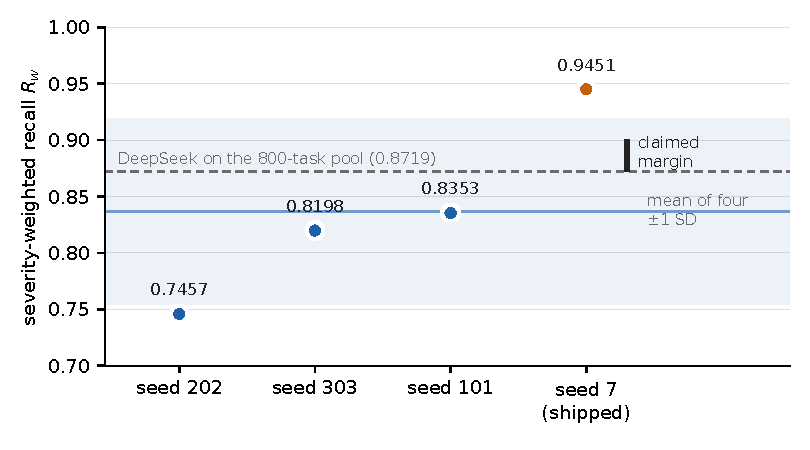
\includegraphics[width=0.7\linewidth]{figures/fig_seeds.pdf}
\caption{$R_w$ for four training seeds of one recipe on the seed-\devPoolSeed{} development pool (\nPoolTasks{} tasks). The shaded band marks the four-run mean plus and minus one SD. The black bar shows the claimed margin \margin{} to scale; DeepSeek's dashed line is its score on the seed-777 pool and is indicative only.}
\label{fig:seeds}
\end{figure}

\begin{table}[t]
\centering\small
\begin{tabular}{@{}lrrrr@{}}
\toprule
Training seed & $R_w$ & Accuracy & Flag prec. & Cost \\
\midrule
202 & 0.7457 & 0.7967 & 0.9057 & 0.267 \\
303 & 0.8198 & 0.8267 & 0.8917 & 0.167 \\
101 & 0.8353 & 0.8233 & 0.8862 & 0.150 \\
7 (shipped) & 0.9451 & 0.8267 & 0.8278 & 0.000 \\
\midrule
mean of four & 0.8365 & & & \\
SD of four & 0.0823 & & & \\
mean of the three fresh runs & 0.8003 & & & \\
SD of the three fresh runs & 0.0479 & & & \\
\bottomrule
\end{tabular}

\caption{Four training seeds of one recipe scored on the seed-\devPoolSeed{} development pool (\nPoolTasks{} tasks). Normalised cost charges escalations and missed HIGH exceptions.}
\label{tab:seeds}
\end{table}

Table~\ref{tab:seeds} and Figure~\ref{fig:seeds} report the four training-seed runs on seed \devPoolSeed{}. Across all four runs, mean $R_w$ is \rwMean{}, standard deviation is \rwSD{} (\sdOverMargin{} times \margin{}, or \sdOverCorrMargin{} times the vote-corrected margin \pubMarginCorr{}), and range is \rwRange{} (\rangeOverMargin{} times the margin). The 95\% chi-square interval on $\sigma$ ($df = 3$) is [\rwSDlo{}, \rwSDhi{}] (one-sided 95\% lower bound \rwSDoneSided{}), and mean minus one SD is \rwMeanMinusSD{}, below DeepSeek's \dsRw{}. Both clauses of the registered screen fire against the claim.

Because the shipped run was selected after beating an earlier sibling run (\rwChampXthree{} vs.\ \rwSiblingXthree{} at three samples on seed 777), including it inflates both the mean and the spread. Across the three unselected fresh runs alone, mean $R_w$ is \rwFreshMean{} (maximum \freshMax{}, sitting \freshGapToDS{} below DeepSeek's seed-777 score) and SD is \rwFreshSD{} (\freshSDoverMargin{} times the margin), with a 95\% chi-square interval ($df = 2$) of [\rwFreshSDlo{}, \rwFreshSDhi{}] that includes the margin. A two-sided one-sample $t$-test of the three fresh runs against DeepSeek's seed-777 score gives $t = $ \tFresh{} ($p = $ \pFresh{}, cross-pool), neither rejecting equality nor supporting the claim. Within the same pool, the shipped run sits \shipGapFresh{} above the unselected mean (\shipGapOverMargin{} times the margin). Under either calculation, the comparison is underpowered at this sample size.

The shipped run's zero-cost HIGH-recall profile also fails to transfer across seeds. Whereas seed 7 caught all \nHigh{} HIGH-severity exceptions at cost \costShipped{}, the three fresh runs incurred normalised costs of \costSeedMidHigh{}, \costSeedMidLow{}, and \costSeedLow{} while achieving higher flag precision (Table~\ref{tab:seeds}), indicating that the training seed shifted the model along the precision--recall frontier.

\subsection{Per-class margin decomposition and memorised-class sensitivity}
\label{sec:perclass}

\begin{table}[t]
\centering\footnotesize
{\setlength{\tabcolsep}{3.5pt}\begin{tabular}{@{}llrrrrrrr@{}}
\toprule
Exception class & Sev. & $w$ & $n$ & E & A & C & $\Delta$(E$-$A) & $\Delta$(E$'-$C) \\
\midrule
\texttt{AMOUNT\_MISMATCH} & HIGH & 1.0 & 73 & 1.000 & 1.000 & 1.000 & +0.0000 & +0.0000 \\
\texttt{FX\_CONVERSION\_ERROR} & HIGH & 1.0 & 32 & 1.000 & 1.000 & 1.000 & +0.0000 & +0.0000 \\
\texttt{BENEFICIARY\_MISMATCH} & HIGH & 0.9 & 42 & 1.000 & 1.000 & 1.000 & +0.0000 & +0.0000 \\
\texttt{COUNTERPARTY\_MISMATCH} & HIGH & 0.9 & 37 & 1.000 & 0.973 & 1.000 & +0.0034 & +0.0000 \\
\texttt{VALUE\_DATE\_MISMATCH} & MEDIUM & 0.6 & 52 & 0.692 & 0.769 & 1.000 & $-$0.0091 & $-$0.0364 \\
\texttt{MISSING\_MESSAGE} & MEDIUM & 0.6 & 45 & 1.000 & 0.978 & 1.000 & +0.0023 & +0.0000 \\
\texttt{DUPLICATE} & LOW & 0.2 & 31 & 0.000 & 0.000 & 0.548 & +0.0000 & $-$0.0129 \\
\texttt{FIELD\_CORRUPTION} & LOW & 0.2 & 37 & 0.270 & 0.270 & 0.270 & +0.0000 & +0.0000 \\
\texttt{PARTIAL\_MATCH} & MEDIUM & 0.5 & 32 & 0.688 & 0.156 & 1.000 & +0.0322 & $-$0.0208 \\
\bottomrule
\end{tabular}
}
\caption{Post hoc nine-class $R_w$ decomposition on the seed-777 pool (\nBench{} tasks, \nExc{} exceptions). Columns E, A, and C give per-class recall for the shipped fine-tune (five samples), DeepSeek base (one sample), and DeepSeek defined-class (five samples); the last two columns give each class's signed contribution to the published margin (E$-$A, total \pubMargin{}) and own-best-prompt margin (E$'-$C, total \bestPrompt{}).}
\label{tab:perclass}
\end{table}

Table~\ref{tab:perclass} decomposes the seed-777 recall margin across all nine exception classes (post hoc, computed from the committed per-task exports). Across all four HIGH-severity classes, both models sit at or near ceiling (DeepSeek A misses one \texttt{COUNTERPARTY\_MISMATCH}; DeepSeek C reaches ceiling on all four). On \texttt{VALUE\_DATE\_MISMATCH}, DeepSeek A already outperforms the fine-tune. The entire published lead comes from \texttt{PARTIAL\_MATCH}: the fine-tune catches \partialChamp{} of \partialN{} tasks against DeepSeek's \partialDS{}, contributing \partialContrib{}---\partialShare{}\% of the \margin{} margin.

That class is memorised from training: the \partialN{} benchmark tasks are generated from \pmPairs{} distinct abbreviation pairs, all \pmShared{} of which appear in the seed-101 training set (\pmTableSize{} pairs in the generator table). Excluding \texttt{PARTIAL\_MATCH} leaves \noPmExcN{} exception tasks across the other eight classes, on which the published margin vanishes (\noPmPub{}, 95\% paired bootstrap CI [\noPmPubLo{}, \noPmPubHi{}]; identical under vote correction). Under the exploratory own-best-prompt and matched-prompt reruns below, DeepSeek's lead persists with or without \texttt{PARTIAL\_MATCH} (\noPmBest{} [\noPmBestLo{}, \noPmBestHi{}] for E$'-$C; \noPmMat{} [\noPmMatLo{}, \noPmMatHi{}] for D$-$C), and DeepSeek C catches all \partialC{} of \partialN{} \texttt{PARTIAL\_MATCH} tasks once the class is defined in its prompt.

\subsection{Trivial floors, matched-prompt reruns, and variance decomposition}
\label{sec:others}
\label{sec:variance}

\begin{table}[t]
\centering\small
\begin{tabular}{@{}lrrr@{}}
\toprule
Policy or model & Accuracy & $R_w$ & Flag F1 \\
\midrule
Always MATCH & 0.5238 & 0.0000 & 0.0000 \\
Always EXCEPTION (AMOUNT\_MISMATCH) & 0.0912 & 0.6673 & 0.6452 \\
Stratified random & 0.2913 & 0.3903 & 0.5181 \\
Base Qwen3-1.7B & 0.6775 & 0.6002 & 0.7173 \\
DeepSeek v4-flash & 0.8762 & 0.8719 & 0.9036 \\
Fine-tuned 1.7B, shipped run & 0.8050 & 0.9007 & 0.8241 \\
Rules oracle (ceiling by construction) & 1.0000 & 1.0000 & 1.0000 \\
\bottomrule
\end{tabular}

\caption{Trivial floors, models, and oracle ceiling on the seed-777 pool (\nBench{} tasks). The oracle is the deterministic verifier that generated the labels and scores $1.0$ by construction.}
\label{tab:floors}
\end{table}

\paragraph{Trivial floors.} Table~\ref{tab:floors} scores input-ignoring policies under the same evaluator. Flagging every pair as \texttt{AMOUNT\_MISMATCH} achieves $R_w = $ \floorRw{} at accuracy \floorAcc{}. The zero-shot base model (\rwBase{}) falls below that constant floor, yielding negative skill (\skillBase{}). Skill-normalised against the constant-flagging floor, the shipped fine-tune leads on $R_w$ (\skillChamp{} vs.\ \skillDS{}) while trailing DeepSeek on flag F1 (\skillFOneChamp{} vs.\ \skillFOneDS{}) and accuracy (\skillAccChamp{} vs.\ \skillAccDS{}). Quoting raw fine-tuning gain over the base model therefore measures from a starting point below a one-line policy.

\begin{table}[t]
\centering\small
\begin{tabular}{@{}cp{6.6cm}rrrr@{}}
\toprule
 & Condition & Accuracy & $R_w$ & Flag prec. & Flag F1 \\
\midrule
A & DeepSeek, shared prompt, 1 greedy sample (as published) & 0.8762 & 0.8719 & 1.0000 & 0.9036 \\
C & DeepSeek, defined-class prompt, 5 samples & 0.9487 & 0.9689 & 1.0000 & 0.9604 \\
E$'$ & Fine-tune, shared prompt, 5 samples (as published, vote corrected) & 0.8050 & 0.8988 & 0.8263 & 0.8252 \\
D & Fine-tune, defined-class prompt, 5 samples & 0.4338 & 0.9401 & 0.5083 & 0.6649 \\
\bottomrule
\end{tabular}

\caption{Exploratory prompt and decode-budget conditions on the seed-777 pool (\nBench{} tasks). Defining every class lifts DeepSeek on every metric while causing the fine-tune to over-flag. Conditions C, D, and E$'$ use decision-level majority voting; A is one greedy sample.}
\label{tab:matched}
\end{table}

\begin{table}[t]
\centering\small
\begin{tabular}{@{}lrr@{}}
\toprule
Paired difference in $R_w$ & Point & 95\% CI \\
\midrule
Published margin, E$-$A & +0.0288 & [+0.0074, +0.0513] \\
Published margin, vote corrected, E$'-$A & +0.0269 & [+0.0064, +0.0493] \\
Same prompt and budget for the frontier model, C$-$A & +0.0970 & [+0.0724, +0.1250] \\
Defined-class prompt for the fine-tune, D$-$E$'$ & +0.0413 & [+0.0228, +0.0624] \\
Matched margin, D$-$C (exploratory) & $-$0.0288 & [$-$0.0432, $-$0.0160] \\
Each model on its own prompt, E$'-$C & $-$0.0701 & [$-$0.0936, $-$0.0481] \\
\bottomrule
\end{tabular}

\caption{Paired differences in $R_w$ with 95\% task-bootstrap intervals (\resamples{} resamples). Matched and own-prompt rows are exploratory on the seed-777 development pool, whose \texttt{PARTIAL\_MATCH} pairs all appear in training (favouring the fine-tune).}
\label{tab:effects}
\end{table}

\paragraph{Matched-prompt and own-best-prompt reruns (exploratory).} The published comparison varied two factors simultaneously: five samples against one, and a prompt naming four classes without defining them. Tables~\ref{tab:matched} and \ref{tab:effects} report the exploratory reruns on seed 777. Supplying DeepSeek with a defined-class prompt and five samples lifts its $R_w$ by \combEffect{} [\combEffectLo{}, \combEffectHi{}] to \rwMatDS{} (accuracy \accMatDS{}, flag F1 \fOneMatDS{}). Under the same prompt, the fine-tune's $R_w$ rises to \rwMatChamp{} only because off-distribution prompting collapses its accuracy to \accMatChamp{} and flag precision to \precMatChamp{} (failing two of five registered guards: flag precision and flag F1), reversing the matched margin to \matMargin{} [\matMarginLo{}, \matMarginHi{}]. Comparing each model on the prompt suited to it at five samples (E$'-$C: fine-tune on its training prompt vs.\ DeepSeek on the defined-class prompt) leaves DeepSeek ahead by \bestPromptAbs{} (\bestPrompt{} [\bestPromptLo{}, \bestPromptHi{}]). One planned cell---DeepSeek with the defined-class prompt and one greedy sample---was not collected because provider credit ran out mid-run, so the \combEffect{} lift cannot be split into prompt-definition and sample-budget components.

\begin{table}[t]
\centering\small
\begin{tabular}{@{}lrlr@{}}
\toprule
Source of variation & Size in $R_w$ & Statistic & $\div$ margin \\
\midrule
Task resampling (redraw 800 tasks) & 0.0483 & CI width & -- \\
Sampling: $\times$3 against $\times$5 on one set of weights & 0.0121 & one difference & 0.42 \\
Evaluation pool (three generator seeds, 300 tasks each) & 0.0115 & SD & 0.40 \\
Training seed (four runs of one recipe) & 0.0823 & SD & 2.86 \\
\bottomrule
\end{tabular}

\caption{Four sources of variation in $R_w$ set against the claimed margin \margin{}. Statistics differ by row and are not directly comparable; task resampling is an interval width rather than an SD.}
\label{tab:variance}
\end{table}

\paragraph{Variance decomposition.} Table~\ref{tab:variance} compares four sources of variation against the \margin{} margin. Evaluation-pool seed (\rwEvalPoolSD{}, \evalPoolOverMargin{} times the margin across seeds \devPoolSeedList{}) and decode-budget change (\rwSamplingMarginal{}, \samplingOverMargin{} times the margin) are modest, and the published task-resampling interval excluded zero. Training-seed variance (\rwSD{}, \sdOverMargin{} times the margin) is the unmeasured component that dominates the comparison.

\subsection{Checkpoint selection and validation-loss decoupling}
\label{sec:ckpt}

\begin{figure}[t]
\centering
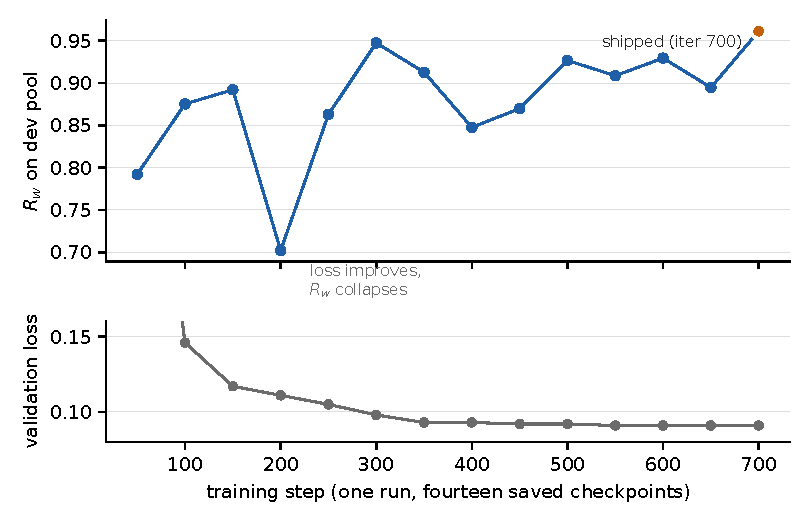
\includegraphics[width=0.7\linewidth]{figures/fig_checkpoints.pdf}
\caption{Fourteen saved checkpoints of the shipped run scored on the development pool (\ckptPoolTasks{} tasks, greedy decoding). Validation loss improves between checkpoints three and four while $R_w$ collapses; inside the loss plateau, $R_w$ varies widely.}
\label{fig:checkpoints}
\end{figure}

Scoring all \nCkpt{} saved checkpoints of the shipped run on the development pool (\ckptPoolTasks{} tasks, greedy decoding; Figure~\ref{fig:checkpoints}) shows that the shipped checkpoint (iter 700, $R_w = $ \rwShippedCkpt{}) was the highest-scoring checkpoint by chance rather than by validation-loss evidence. Validation loss and $R_w$ correlate negatively across checkpoints (tie-corrected Spearman $\rho = $ \ckptRho{}). $R_w$ spans \ckptSpread{} (\ckptSpreadX{} times the margin) across the trajectory and \plateauSpread{} (\plateauSpreadX{} times the margin) across the \plateauN{} checkpoints rated identically by validation loss; between steps 150 and 200, validation loss improved from \lossBefore{} to \lossAfter{} while $R_w$ collapsed from \rwBefore{} to \rwAfter{}.

\section{Diagnostic checklist for fine-tuning comparisons}
\label{sec:instrument}

Each check below costs a small fraction of a fine-tuning project and catches one of the failure modes observed here before publication:
\begin{enumerate}\setlength\itemsep{1pt}\setlength\parskip{0pt}
\item \textbf{Measure training-seed spread before quoting a margin.} At the four-run SD (\rwSD{}) and margin (\margin{}), an 80\%-power two-sided test at $\alpha = 0.05$ requires roughly \seedsNeeded{} training runs; at the three-run unselected SD (\rwFreshSD{}), roughly \seedsNeededFresh{} runs. Margins this small cannot be established from a handful of runs.
\item \textbf{Name the variance component the confidence interval excludes.} A task-resampling bootstrap quantifies evaluation-item noise only; recipe-level claims require retraining variance.
\item \textbf{Decompose the margin by class.} A per-class contribution table (Table~\ref{tab:perclass}) exposes single-class memorization immediately.
\item \textbf{Report trivial floors beside raw gains.} Comparing against constant-flagging and stratified-random policies prevents measuring improvement from a negative-skill baseline.
\item \textbf{Match comparator prompts and decode budgets, or report own-best-prompt pairs.} Unequal prompts and voting budgets confound model quality with harness effort.
\item \textbf{Score every checkpoint on a separate validation pool.} Validation-loss plateaus do not preserve task-specific recall metrics.
\item \textbf{Freeze and reserve a single-use test pool.} Development-pool selection inflates margins; confirmatory verdicts require an untouched pool scored once.
\end{enumerate}

\section{Limitations}
\label{sec:limits}

\begin{itemize}\setlength\itemsep{1pt}\setlength\parskip{0pt}
\item \textbf{Small seed count and missing per-task exports.} Only four runs enter the seed spread (three unselected; an earlier sibling run's weights were overwritten). Per-task exports and generating scripts for the three fresh runs were not committed in this repository, so Table~\ref{tab:seeds} relies on committed summary JSONs, and validation cadence differed from the shipped run. With $df = 2$ or $3$, $\sigma$ is imprecisely estimated; the study shows the comparison is underpowered rather than establishing the true recipe mean.
\item \textbf{Cross-pool comparison.} The seed runs were scored on seed \devPoolSeed{} (\nPoolTasks{} tasks), whereas the headline and DeepSeek were scored on seed 777 (\nBench{} tasks). The same shipped weights shift by \poolShift{} (\poolShiftOverMargin{} times the margin) between seed 777 (\rwChampPoolBench{}) and seed \devPoolSeed{} (\rwShipped{}), and sit \poolMeanShift{} below the mean of three development pools (range \evalPoolRange{}). DeepSeek was not scored on seed \devPoolSeed{}, so cross-pool comparisons are indicative only; the within-pool gap (\shipGapFresh{}) needs no cross-pool assumption.
\item \textbf{Exploratory reruns and unscored frozen pool.} The matched-prompt and own-best-prompt reruns ran on the seed-777 development pool (with 100\% \texttt{PARTIAL\_MATCH} pair overlap favouring the fine-tune), and condition B (DeepSeek defined-class prompt, one sample) was not collected. The frozen seed-\frozenSeed{} pool (\nFrozen{} signatures) remains unscored; a confirmatory protocol is drafted in \texttt{docs/DESIGN-V2.md}.
\item \textbf{Synthetic similarity and single-generator scope.} Although exact-signature train--eval overlap is \exactOverlap{}, a MinHash audit places \nearDup{} of \nBench{} tasks (\nearDupPct{}\%) at Jaccard similarity $\ge$ \nnHigh{} and \nMidBand{} between \nnFloor{} and \nnHigh{} (removing the \nearDup{} near-duplicates shifts the margin by \dedupShift{}). All results cover one model size (1.7B), one synthetic generator, and one unpinned API comparator scored across separate dates; task bootstraps treat the \partialN{} \texttt{PARTIAL\_MATCH} tasks as independent despite sharing \pmPairs{} name pairs, and the oracle ceiling of $1.0$ holds by verifier construction.
\item \textbf{Pre-registration provenance and local tag.} \texttt{PRE-REGISTRATION.md} carries no external third-party timestamp and was written after viewing two initial runs; guard thresholds were calibrated to catch collapse relative to the shipped model (Appendix~\ref{app:provenance}).
\end{itemize}

\section{Conclusion}
\label{sec:conclusion}

A single-run \margin{} recall advantage for a 1.7B LoRA fine-tune over DeepSeek v4-flash does not survive basic variance and attribution checks. Training-seed standard deviation is \rwSD{} across four runs (\rwFreshSD{} across three unselected runs), leaving the comparison underpowered; \partialShare{}\% of the margin comes from one memorised class whose removal eliminates the lead (\noPmPub{}); matching prompt definitions and five-sample voting reverses the margin to \matMargin{} (\bestPrompt{} on own-best prompts); a constant-flagging policy beats the base model (\floorRw{} vs.\ \rwBase{}); and validation loss correlates negatively with $R_w$ across checkpoints ($\rho = $ \ckptRho{}). The previously published headline is retracted. Obtaining a confirmatory verdict requires scoring ten or more fresh training seeds alongside matched and own-best-prompt frontier comparators on the untouched frozen seed-\frozenSeed{} pool with held-out abbreviation pairs (\texttt{docs/DESIGN-V2.md}).

\section*{Disclosures and availability}

The code, analysis scripts, and manuscript were written with an AI coding assistant under the authors' direction and review; every measured number is generated from committed artifacts by \texttt{paper/build\_assets.py} and verified by automated tests. The first author works on a commercial AI gateway; nothing from that product, employer, or its customers is used here, and all data are synthetic. Code and artifacts are licensed Apache-2.0 at \url{https://github.com/caiotheodoro/reconforge} (the shipped adapter weights are hosted on Hugging Face); this paper is licensed CC BY 4.0 and has not been peer reviewed. Work on the repository began on 2026-08-07; the first preprint version (\texttt{paper-v1.0}, Zenodo record 24455455) was compiled and deposited on 2026-11-23, and this revision (\texttt{paper-v2.0}) is of 2026-11-23. Per-task exports under \texttt{docs/validation/} reproduce every published, matched, own-best-prompt, and per-class figure; second-round training-seed scripts and per-task exports for the three fresh seeds remain uncommitted as noted in \S\ref{sec:limits}.

{\small
\bibliographystyle{plainnat}
\bibliography{refs}}

\appendix

\section{Pre-registration provenance, retraction record, and analysis corrections}
\label{app:provenance}

\paragraph{Timeline and registration clock.} The repository was created on 2026-08-07; the initial three-sample headline was published on 2026-08-08, restated at five-sample voting on 2026-08-27 alongside the committed seed-\frozenSeed{} frozen-test signatures (the only external GitHub timestamp prior to the 2026-11-23 paper release), and followed by \texttt{PRE-REGISTRATION.md} on 2026-08-29 (tagged locally with an unsigned annotated tag and one same-day background-number amendment). Between 2026-09-05 and 2026-11-23 the public README still carried the un-retracted headline while the retraction lived in a local working copy; the 2026-11-23 release and Zenodo deposit constitute the first public retraction record.

\paragraph{Corrections identified during internal review.} Independent checks and reruns caught six defects in earlier drafts and repository summaries, all corrected in the committed artifacts and this paper:
\begin{enumerate}\setlength\itemsep{1pt}\setlength\parskip{0pt}
\item \textbf{Vote-rule mismatch.} Apparent symmetry between the published margin (\pubMargin{}) and matched margin (\matMargin{}) came from comparing whole-dict voting against decision-level voting; under one rule the published margin is \pubMarginCorr{}.
\item \textbf{Exclusion of the shipped run from seed spread.} An earlier draft excluded seed 7 on the unchecked assumption that validation cadence altered the RNG stream; both four-run (\rwSD{}) and three-run unselected (\rwFreshSD{}) spreads are now reported side by side.
\item \textbf{Guard failure count.} Failed guards under the matched prompt were previously miscounted as three of five (one guard split across two rows, another omitted); the true count is two of five (flag precision and flag F1).
\item \textbf{Class share denominator.} The \texttt{PARTIAL\_MATCH} share was previously quoted as \partialShareXthree{}\% (its share of the three-sample margin) rather than \partialShare{}\% of the five-sample margin.
\item \textbf{Cause of missing condition B.} An earlier draft speculated that greedy decoding overran a token budget; the actual cause was exhausted API credit.
\item \textbf{Tied-rank correlation.} Validation-loss Spearman $\rho$ was corrected with tie handling to \ckptRho{}.
\end{enumerate}

\end{document}
